\subsubsection{buffer的设计与实现}
多核下的MapReduce模型中,
Map阶段产生的key-value,都存放于一个共享的中间结构,
之前的很多研究都显示,
影响多核MapReduce系统性能的关键因素是
对该中间结构的操作效率\cite{mao2010metis}。

Phoenix中map插入key-value的过程为:
map根据hash(key)确定key在二维数组中的位置,
具有相同hash值的多个key存于一个array中,
通过折半查找,确定key在array中的位置,最后插入。
多个map产生的相同key会存于同一列。
reduce会对二维数组中的每一列中key的多个value进行归并,
得到最终结果。


从Phoenix处理中间数据的流程可以看出,
Phoenix中key-value需要保持有序,
便于Reduce阶段的归并。
Map阶段需要完成map计算以及key的查找、插入,
Reduce阶段只需要简单的进行归并。

通过分析Phoenix中间结构,以及中间结构设计存在的局限性,
DMR试图从两个角度对Phoenix的中间结构进行改进:
\begin{itemize}
  \item 改进Phoenix中的公有buffer,
  每个map线程都拥有自己私有的buffer,
  这样可以避免Map和Reduce之间的barrier,
  增加并行的程度。
  \item 针对DMR本身设计的特点,
  优化buffer的内部实现,
  不再使用hash表的方式组织key,
  而是采用array表。
\end{itemize}
以下将详细解释私有buffer的设计与优化。

为了避免Map和Reduce之间的barrier,
DMR将Phoenix中共享的中间结构拆分,
每个map worker拥有一个local buffer pool,
buffer池中有多个buffer,
分别用于存放特定reduce的数据如图\ref{dmr:buffers}。
\begin{figure}[!h!t]  
    \centering
    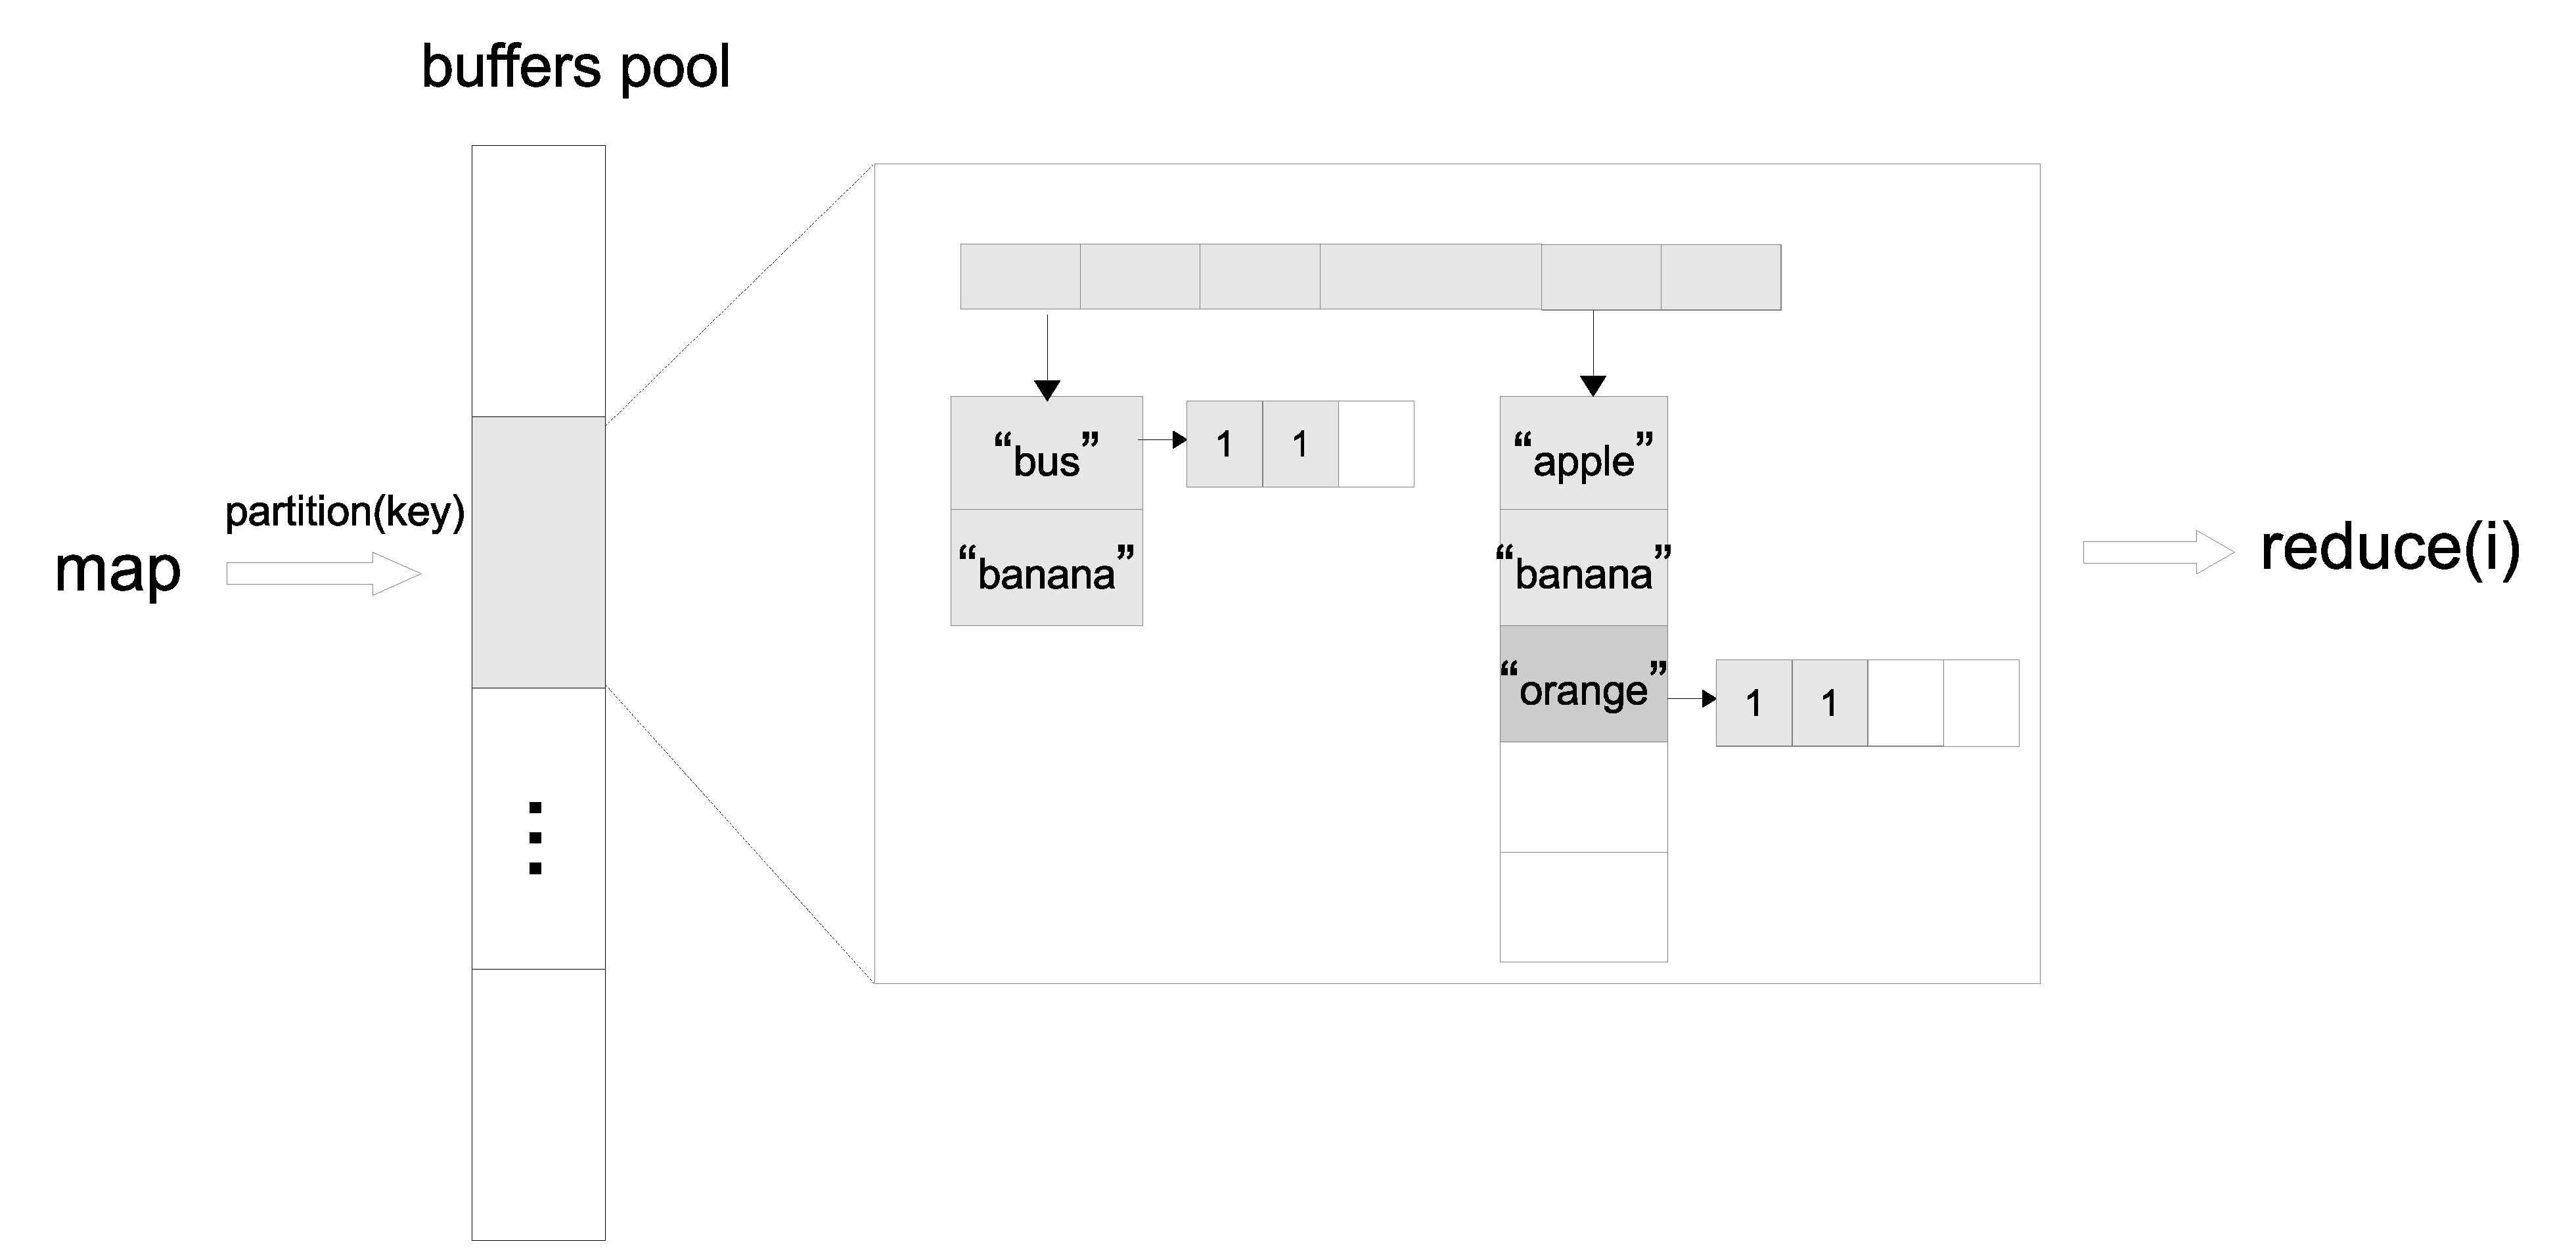
\includegraphics[width=0.7\textwidth]{img/dmr_buffers.eps}
    \caption{local buffer pool for each map worker}
    \label{dmr:buffers}
\end{figure}

DMR中map和reduce之间数据流动的过程为:
map产生key-value,
根据partition(key)确定buffers pool中的某个buffer,
当该buffer中的key-value达到预先设定的阈值时,
map触发物理内存的重映射,
reduce开始读取该buffer中的数据,
开始reduce的工作。

buffer的内部实现,
采用类似Phoenix的方式,即hash表的方式进行组织。
在map阶段开启combiner,
以减少内存和动态内存分配带来的开销。
采用hash表组织的优势在于:
key的查找长度比较短。

\begin{figure}[!h!t]  
    \centering
    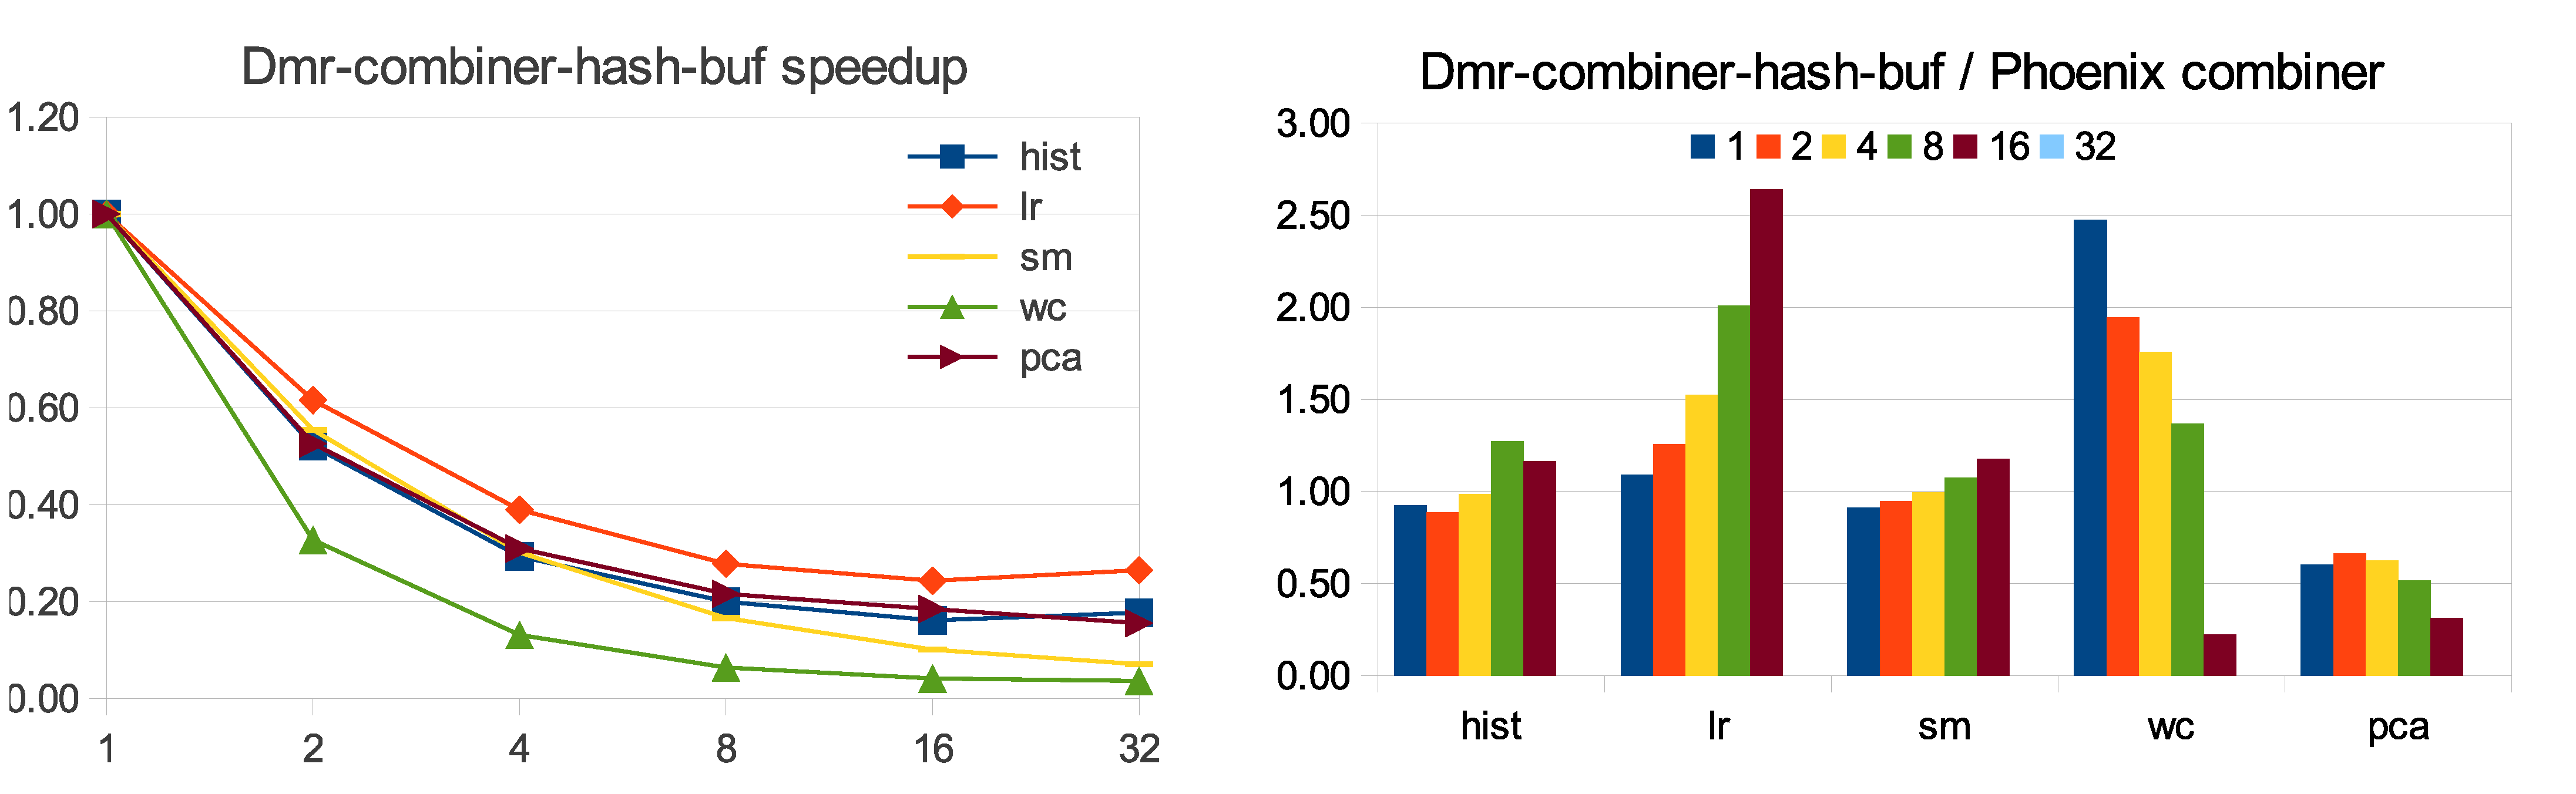
\includegraphics[width=1\textwidth]{img/dmr_time_hash.eps}
    \caption{dmr compare to phoenix}
    \label{dmr:time-hash}
\end{figure}

改进后的实验结果如图\ref{dmr:time-hash}显示,
左图表明,随着核数的增多,性能较平稳;
右图为DMR与Phoenix的对比结果,
其中hist, pca, sm,DMR具有较好的性能,
但结果并不理想,
为此,我们需要分析DMR-hash实现的局限,
充分利用DMR处理流程的特点,
以改进性能。


DMR-hash的buffer中,
每个buffer是hash表的方式实现,
其中存放的key-value数据的分布是离散的,
然而Producer-Consumer模型要求key-value存放
于一块连续的物理空间中。
因此,hash buffer在出发重新映射之前
首先需将分散的key-value汇集到一块连续的空间中,
通常是数组,我们称这个过程为group阶段。
通过实验的数据发现,group的开销相当大。
此外,hash buffer的方式,需要大量的动态内存分配。

针对DMR中Map和Reduce阶段并行这一特点,
我们试图改进buffer的hash实现。
它不再采用原来Phoenix中的hash表的组织方式,
而是采用更简单的array,
map worker产生的key-value只需追加到array中即可,
无需排序。
同时reduce阶段也可以开启combiner.
通过array实现会带来以下优势:

\begin{itemize}
  \item 初始化array buffer时,
  运行时为其分配一块固定大小的空间,
  该预分配的空间可重复利用,
  可减少动态内存分配带来的开销。
  
  \item 相较于hash buffer,
  array buffer是一块连续的空间,
  因此可以避免group带来的开销。
  
  \item 由于L1 cache的大小有限,
  group阶段在遍历时,
  会更大的可能性访问不在L1 cache中的key-value;
而array buffer不需要group阶段,
因此会更少的cache miss.
如图\ref{dmr:hash-to-array}左图所示。
从而array buffer可有效提高性能
\end{itemize}


\begin{figure}[!h!t]  
    \centering
    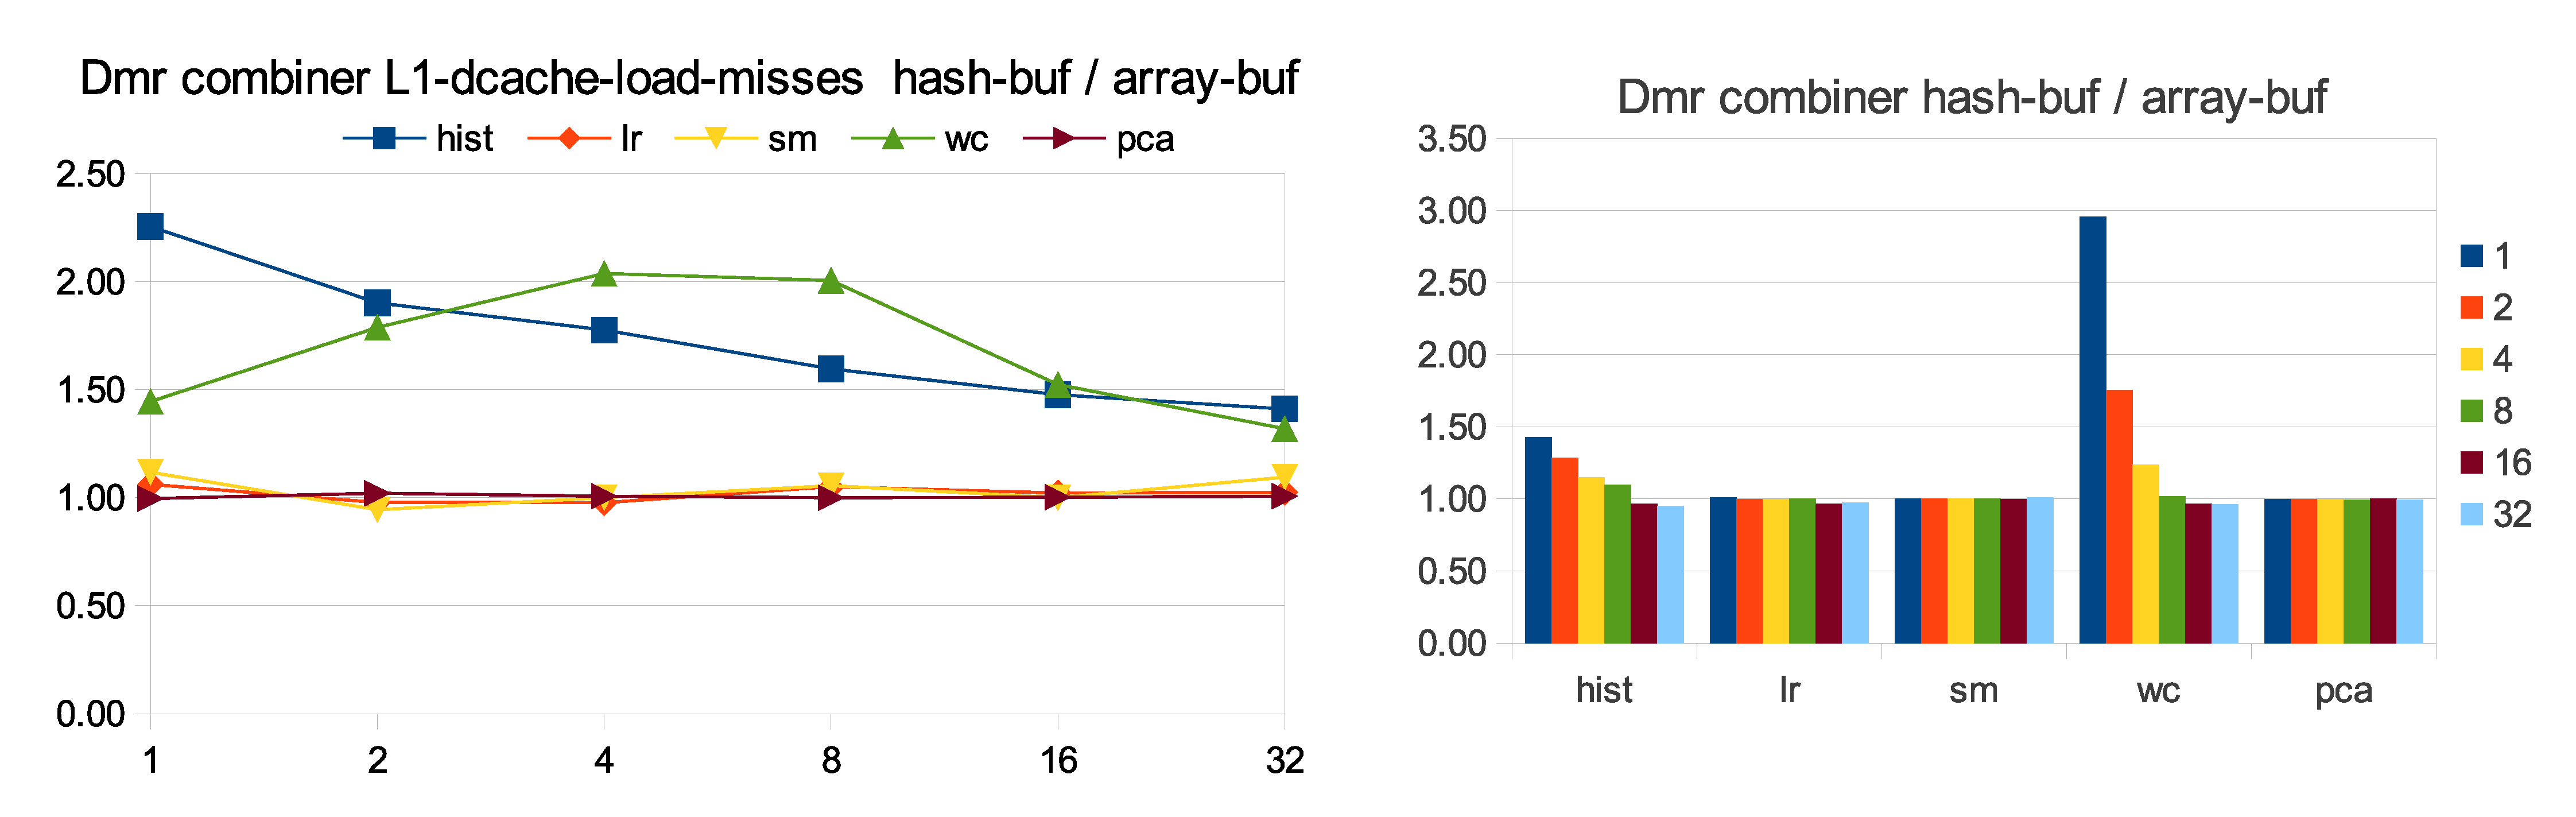
\includegraphics[width=1\textwidth]{img/dmr_hash_to_array.eps}
    \caption{hash compare to array}
    \label{dmr:hash-to-array}
\end{figure}


优化后DMR与Phoenix对比的整体性能如图\ref{dmr:time-array}
\begin{figure}[!h!t]  
    \centering
    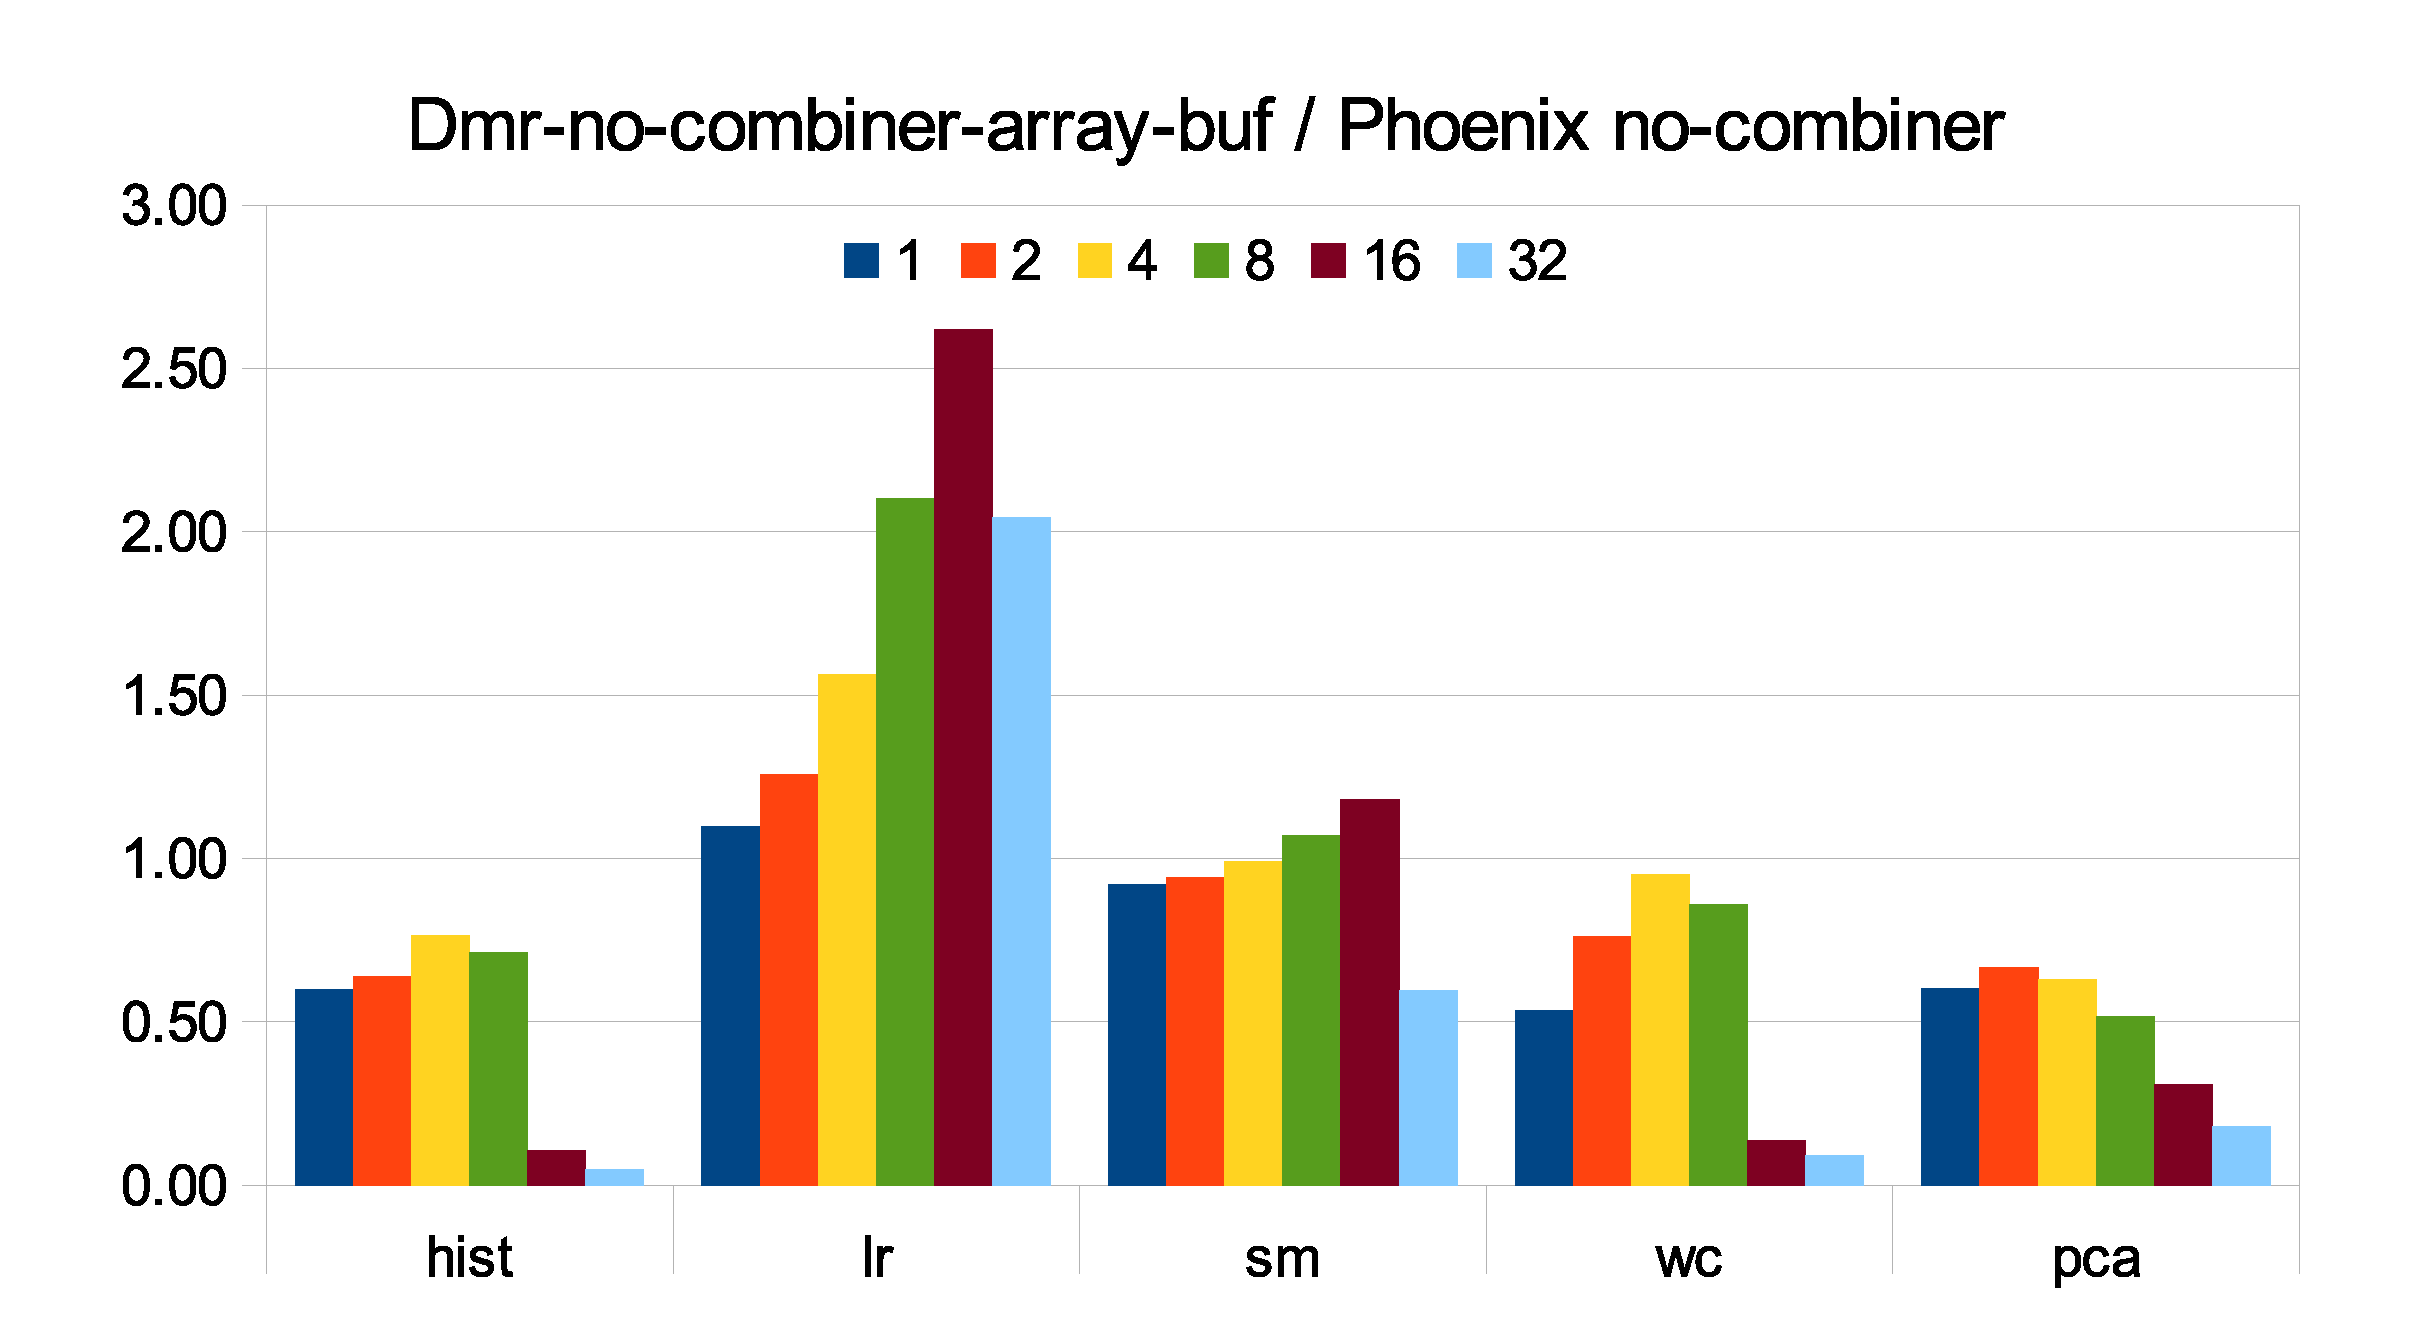
\includegraphics[width=0.5\textwidth]{img/dmr_time_array.eps}
    \caption{dmr compare to phoenix}
    \label{dmr:time-array}
\end{figure}
